
% !TEX TS-program = pdflatex
% !TEX encoding = UTF-8 Unicode
 
\documentclass[twoside]{report} % use larger type; default would be 10pt
%\documentclass{report}
 
\usepackage[utf8]{inputenc} % set input encoding (not needed with XeLaTeX)
 
%%% Examples of Article customizations
% These packages are optional, depending whether you want the features they provide.
% See the LaTeX Companion or other references for full information.
 
%%% PAGE DIMENSIONS
\usepackage{geometry} % to change the page dimensions
\geometry{a4paper} % or letterpaper (US) or a5paper or....
\geometry{margin=1in} % for example, change the margins to 2 inches all round
%\geometry{landscape} % set up the page for landscape
\geometry{portrait}
%read geometry.pdf for detailed page layout information
 
\usepackage{graphicx} % support the \includegraphics command and options
 
% \usepackage[parfill]{parskip} % Activate to begin paragraphs with an empty line rather than an indent
 
%%% PACKAGES
\usepackage{booktabs} % for much better looking tables
\usepackage{array} % for better arrays (eg matrices) in maths
\usepackage{paralist} % very flexible & customisable lists (eg. enumerate/itemize, etc.)
\usepackage{verbatim} % adds environment for commenting out blocks of text & for better verbatim
\usepackage{subfig} % make it possible to include more than one captioned Figure/table in a single float
\usepackage{amsmath}
\usepackage{gensymb}
\usepackage{csquotes}
% These packages are all incorporated in the memoir class to one degree or another...
 \graphicspath{{Figures/}}
%%% HEADERS & FOOTERS
\usepackage{fancyhdr} % This should be set AFTER setting up the page geometry
\pagestyle{fancy} % options: empty , plain , fancy
\renewcommand{\headrulewidth}{0pt} % customise the layout...
\lfoot{}\cfoot{\thepage}
 
\rfoot{}
 
%%% SECTION TITLE APPEARANCE
\usepackage{sectsty}
\allsectionsfont{\sffamily\mdseries\upshape} % (See the fntguide.pdf for font help)
% (This matches ConTeXt defaults)
 
 
%%% END Article customizations
 
%%% The "real" document content comes below...
 
\title{\bf AE 3340 Individual Project\\}
\author{\bf Micaiah Smith-Pierce\\
903328232\\
}
\date{\it 28 November, 2018} % Activate to display a given date or no date (if empty),
 
         % otherwise the current date is printed 

\usepackage{graphicx}
 
\begin{document}
\maketitle
\cleardoublepage
 
\tableofcontents
\cleardoublepage

\chapter{Unconstrained Optimization}

\section{Problems 1, 2, and 3}
The first three problems are analytic, so I did them by hand. They may be found on the following four pages.
\cleardoublepage
\section{Problem 4}
Both Newton and Quasi-Newton methods essentially suppose that the objective function is quadratic, and then guess
where the minimum is (or potentially which direction it is in). Although the assumption that the function is quadratic
may seem arbitrary, in fact there is a good reason why it makes sense to assume that the function is quadratic, and
nothing else. The reason is that the quadratic functions are the simplest ones which can actually have a minimum (without
constraints). A linear function never has a strong minimum, and a cubic, or transcendental function would be unnecessarily
complicated. So, an algorithm which can approximate the objective as a quadratic function is using the least possible amount
of complexity and information in order to guess the location of the minimum. This is in contrast to the steepest descent method,
which does not actually guess the location of the minimum, but simply attempts to decrease the objective as much as possible
locally.

Moreover, both Newton and Quasi-Newton methods utilize the Hessian matrix, as well as the gradient. The Hessian matrix is the
generalization of the second derivative of single-variable functions to multiple variables. Thus, just as the $\nabla$ operator
is the generalization of the derivative, the Hessian matrix $H$ for a function $f(\bf x)$ can be defined in terms of $\nabla$ and
the vector outer product as:
\[ H = \nabla \nabla^T f(\bf x) \]
If, at a point $\bf x_0$, $f(\bf x_0)$, $\nabla f(\bf x_0)$, and $H$ are known, and the function is assumed to be quadratic, then
the location of the minimum, $\bf x^*$ is known, and can be calculated as:
\[ \mathbf{x^*}-\mathbf{x_0} = -H^{-1} \nabla f(\bf x_0) \]
As stated in the MATLAB documentation. Here, the $^{-1}$ denotes the matrix inverse. Realistically, however, the quadratic
approximation may not be particularly accurate, so for a highly nonlinear function, $ \mathbf x^*$ may not be very close to the actual
minimum unless $\mathbf x_0$ is already close enough to the minimum that the higher-order derivatives do not significantly affect the
behavior of the function. For that reason, rather than attempt to jump straight to the minimum, it may be advantageous to simply
approximate the \textit{direction} to the minimum, so that a standard line-search method can be used. In this case, the following
similar equation gives the direction $\mathbf{d}$ toward the minimum of the quadratic approximation:
\[ \mathbf{d} = -H^{-1} \nabla f(\bf x_0) \]

The only difference between the Newton and Quasi-Newton methods is how the Hessian is computed (or estimated). The Newton
method simply assumes that the Hessian is known, which means it must be computed either analytically, or using finite differences,
i.e. sampling the function at points near $\bf x_0$ in order to build a quadratic approximation. This can cost a lot of computation
time if the function is expensive to evaluate, or the number of variables is large. For $n$ variables, $n^2$ points must be sampled
to compute the Hessian by finite differences. The Quasi-Newton method solves this problem by using information from prior iterations
of the algorithm. Rather than sample $n^2$ new points at every iteration, it builds the quadratic approximation of $f$ using the value
of $f$ at each previous point that the search has visited. With each iteration, it updates its previous estimate of the Hessian
using the changes in the objective function's gradient. In this way, none of the information from previous iterations is wasted,
which usually makes the algorithm more efficient.

\section{Problem 5}
\subsection{Part a}
The analytic gradient is clearly performs better than the estimated derivatives in all respect, and the steepest descent performs
dramatically worse than either of the other two. The steepest descent algorithm only moves by extremely tiny increments, which is
probably because the search direction does not take into account the curvature of the function. All of the search algorithms follow
a curved path, but the steepest descent essentially must repeatedly stop to change directions, whereas the other two algorithms
must do so less often, because the search direction anticipates the curvature of the path. So, the steepest descent algorithm
ends up with more
iterations and more function evaluations.

The estimated gradients method and analytic gradients method appear similar. However, the path that the estimated gradients takes
utilizes shorter steps, and ``zigzags'' more than the analytic gradients. This is probably because the estimate of the gradient
is not as accurate as the analytic computation, so the search direction is subject to additional change, essentially because
of unceratianty in the gradient computation. The estimated gradients method takes modestly more iterations to reach the solution,
but it has nearly five times the number of function evaluations. This is probably because it must perform additional function
evaluations during each iteration for the sole purpose of estimating the derivatives, which is completely unnecessary for the
analytic gradient method.

\subsection{Part b}
Both the estimated and analytic gradient methods performed better in this case. This is probably because the starting point
was located such that the algorithms did not have to perform as many iterations in the ``valley'', which is the most challenging
area. Yet, the most interesting thing about this example is that the analytic gradient took a completely different path
from the estimated gradients function. The estimated gradients algorithm began searching straight down (toward the origin),
whereas the analytig gradients took a path which is more in the positive x-direction. This is probably because the gradient vector was
not perfectly vertical, which was detected and exploited by the analytic gradients algorithm, whereas the estimated gradients
algorithm did not compute the gradient precisely enough to detect the asymmetry.

\chapter{Constrained Optimization}
\section{Problem 6}

\textbf{Note}: Since computer code is inherently nondimensional, the problem is specified without
units. In addition, let b and c be in feet.


\textbf{Minimize:}
\[ f(b,c) = -\frac{L}{D} \]

\textbf{Subject to:}
\[ g_1(b,c) = b - 10c \leq 0\]
\[ g_2(b,c) = \frac{8000}{bc} - 40 \leq 0\]
\[ g_3(b,c) = b - 55 \leq 0 \]

\section{Problem 7}
Figure \ref{LonDplot} below is my response to problem 7, parts a and b.

\begin{figure}
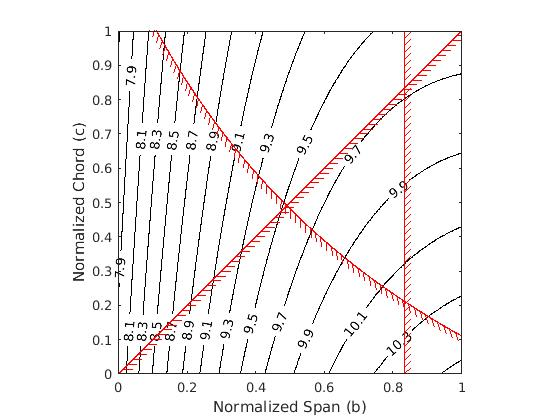
\includegraphics[width = \linewidth]{LonDplot.jpg}
\centering
\caption{Answer to problem 7.}
\label{LonDplot}
\end{figure}

\cleardoublepage

\section{Problem 8}
\begin{tabular}{p{0.3\linewidth}|p{0.3\linewidth}|p{0.3\linewidth}}
Algorithm & Iterations & Function Evaluations \\
\hline
interior-point & 12 & 42 \\
trust-region-reflective & Failed & Failed \\
sqp & 7 & 24 \\
sqp-legacy & 7 & 24 \\
active-set & 4 & 15 \\
\end{tabular}
\\

The active-set algorithm was most efficient in terms of function evaluations. This agrees with the documentation,
which seems to state that active-set is exceptionally fast in situations it is suited for.

\section{Problem 9}
\subsection{Parts a - f}
My response to parts a through f can be found on the following two handwritten pages.
\cleardoublepage
\subsection{Part g}
Yes, all of the KKT conditions are satisfied to an acceptable level of numerical precision. There are three KKT conditions.
The first is that $\bf x^*$ must be feasible. I clearly showed that this condition is met in part a. The second is that
for any $j$, $\lambda_j g_j(\mathbf{x^*}) = 0$. I showed this in part d. The final condition is that
$\nabla_{\mathbf{x}}\mathcal{L}(\mathbf{x^*,\lambda}) = \mathbf{0}$ (for the appropriate definition of $\mathcal{L}$). I
demonstrated this in part f. So, it has already been established that all three conditions are satisfied.

\section{Problem 10}
The vectors are plotted in Figure \ref{equal_and_opposite}. It is apparent from this plot that $\nabla \mathcal{L} = \mathbf{0}$
because the vector $\lambda_1 \nabla g_1$ is equal in magnitude and opposite in direction from $\nabla f$. So,
$\nabla \mathcal{L}$, which in this case is the sum of these two vectors, must be zero.

\begin{figure}
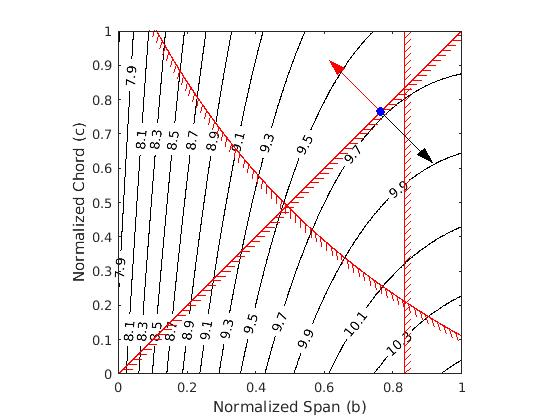
\includegraphics[width = \linewidth]{equal_and_opposite.jpg}
\centering
\caption{The vectors $\nabla f$ (black) and $\lambda_1 \nabla g_1$ (red) at the computed minimum.}
\label{equal_and_opposite}
\end{figure}


\end{document}
